%!TEX program = xelatex
\let\stop\empty

\documentclass[12pt,a4paper]{exam-zh}

\usepackage{xeCJK}
% \setCJKmainfont{NSimSun}
\setCJKmainfont{Noto Serif CJK SC}
\usepackage{geometry}
\usepackage{array}
\usepackage{tikz}
\usepackage{amsmath}
\usepackage{wrapfig}
\usepackage{adjustbox}
\usepackage{enumitem}
\usepackage{fancyhdr}
\usetikzlibrary{quotes,angles}
\usetikzlibrary{calc}
\usepackage{scalerel}
\def\mcirc{\mathbin{\scalerel*{\circ}{j}}}
\def\msquare{\mathord{\scalerel*{\Box}{gX}}}

% \renewcommand{\choiceshook}{%
%     \setlength{\leftmargin}{18pt}%
% }
\geometry{margin=2cm}
\AtBeginDocument{\zihao{4}}


%region ----------- 调整 exam -----------
\examsetup{
    % problem/label = \arabic*., 
    % 设置大题题号格式 
        problem = {
        top-sep = 1em,      % 题头上方的间距（默认 0.25em）
        bottom-sep = 1em,   % 题号下方的间距（默认 0pt）
    },
    % 隐藏大题后的分值显示 
    problem/show-points = false,
    % 调整各 question 之间的垂直间距
    question = {
        top-sep = 1em,
        bottom-sep = 1em,
    },
    % 调整小题列表的缩进和间距
    list/step-name = {}, 
    solution = {
    show-solution = show-move, % 答案自动移动到卷末
    label-content = {参考答案},  % 答案区的标题文字
    show-qed = true            % 在解答末尾显示结束符号 ◻ 
  },
    page = {
    size = a4paper,           % 设定纸张大小 
    foot-content = { - ; - }  % 页脚显示为 -1-, -2- 格式 
  }
}
\setlist[enumerate,1]{
    label=(\alpha*), 
    itemsep=0.5em, 
    leftmargin=2em, 
    after=\hfill % 配合您之前要求的百分比靠右样式
}
%endregion


% ==========================
% 卷面变量设置（只需改这里）
% ==========================
% ==========================
% 卷面变量设置（只需改这里）
% ==========================
\newcommand{\paperlevel}{初中二}
\newcommand{\papersubject}{数学 试卷二}
\newcommand{\schoolname}{金宝培元独立中学}
\newcommand{\examname}{八月考}
\newcommand{\classinfo}{J2(H / I/ F)}
\newcommand{\examdate}{5-8-2026}
\newcommand{\examtime}{11:00-12:15}
\newcommand{\questiontotal}{5}
\newcommand{\paperpercentage}{60\%}
\newcommand{\setterteacher}{蔡杰庆师}
\newcommand{\reviewteacher}{谢明政师}
\newcommand{\auditteacher}{雷泳健师}

\begin{document}


%region 三栏标题区
% ==========================
\noindent
\begin{tabular*}{\textwidth}{@{\extracolsep{\fill}} p{0.3\textwidth} p{0.35\textwidth} p{0.3\textwidth}}

\raggedright
\textbf{\paperlevel}\\[0.2em]
\textbf{}{\papersubject}\\[0.4em]
姓名：\underline{\hspace{3cm}} &

\centering
\textbf{\schoolname}\\[0.2em]
\textbf{\examname}\\[0.4em]
班级：\classinfo &

\raggedright
日期：\examdate\\[0.2em]
时间：\examtime\\[0.4em]
得分：\underline{\hspace{2.5cm}} \\

\end{tabular*}

\begin{flushleft}
作答题：\questiontotal 题全做（\paperpercentage） 
\end{flushleft}
%endregion



%region 范围：初中数学-进位制 | 考点：二、八、十进制换算与四则运算 | 难度：中等
\begin{question}[points = 12]
    \begin{enumerate}[label=(\alph*)]
        \item 将 $91$ 分别化为二进数与八进数。 \hfill (3\%)
        \item 计算 $1011011_2 + 231_8$（答案用十进数表示）。 \hfill (6\%)
        \item 计算 $101_2 \times 11_2$。 \hfill (3\%)
    \end{enumerate}
\end{question}

\begin{solution}
    \begin{enumerate}[label=(\alph*)]
        \item 将 $91$ 分别化为二进数与八进数。 \\
        用"除基数取余法"反复相除并记录余数。
        \[
            91 = 1011011_2
        \]
        \hfill (1分)
        \[
            91 = 133_8
        \]
        \hfill (2分)

        \item 计算 $1011011_2+231_8$（答案用十进数表示）。 \\
        分别将两数转换为十进数后相加。
        \begin{align*}
            1011011_2 &= 64+16+8+2+1 = 91 \\
            231_8 &= 2\times64+3\times8+1 = 153
        \end{align*}
        \hfill (4分)
        \[
            91+153 = 244
        \]
        \hfill (2分)

        \item 计算 $101_2 \times 11_2$。 \\
        转换为十进数相乘后再转回二进数。
        \[
            101_2 \times 11_2 = 5 \times 3 = 15
        \]
        \hfill (1分)
        \[
            15_{10} = 1111_2
        \]
        \hfill (2分)
    \end{enumerate}
\end{solution}
%endregion


%region 范围：初中数学-代数式 | 考点：去括号合并同类项、分式化简 | 难度：中等
\begin{question}[points = 12]
    \begin{enumerate}[label=(\alph*)]
        \item 化简：$1-\{1-[1-(1-x)-x]-x\}-x$。 \hfill (4\%)
        \item 若 $a=3,\ b=1$，求 $\dfrac{a}{a-b} - \dfrac{b}{a+b}$ 的值。\hfill (4\%)
        \item 化简：$\dfrac{2x-3}{9} + \dfrac{x+2}{6} + \dfrac{5x+8}{12}$。 \hfill (4\%)
    \end{enumerate}
\end{question}

\begin{solution}
    \begin{enumerate}[label=(\alph*)]
        \item 化简 $1-\{1-[1-(1-x)-x]-x\}-x$。 \\
        由内向外逐层去括号。
        \[
            1-(1-x) = x
        \]
        \hfill (1分)
        \[
            1-x-x = 1-2x \quad (\text{方括号内})
        \]
        \hfill (1分)
        \[
            1-(1-2x)-x = x \quad (\text{花括号内})
        \]
        \hfill (1分)
        \[
            1-x-x = 1-2x \quad (\text{最外层})
        \]
        \hfill (1分)

        \item 若 $a=3,\ b=1$，求 $\dfrac{a}{a-b}-\dfrac{b}{a+b}$ 的值。 \\
        先通分化简为单一分式，再代入数值。
        \[
            \frac{a}{a-b}-\frac{b}{a+b} = \frac{a(a+b)-b(a-b)}{(a-b)(a+b)} = \frac{a^2+b^2}{a^2-b^2}
        \]
        \hfill (2分)
        \[
            = \frac{9+1}{9-1} = \frac{5}{4}
        \]
        \hfill (2分)

        \item 化简 $\dfrac{2x-3}{9}+\dfrac{x+2}{6}+\dfrac{5x+8}{12}$。 \\
        求三个分母的最小公倍数 $36$ 作为公分母，通分后合并同类项。
        \[
            \frac{4(2x-3)+6(x+2)+3(5x+8)}{36}
        \]
        \hfill (2分)
        \begin{align*}
            8x-12+6x+12+15x+24 &= 29x+24 \\
            \implies \text{原式} &= \frac{29x+24}{36}
        \end{align*}
        \hfill (2分)
    \end{enumerate}
\end{solution}
%endregion


%region 范围：初中数学-多边形 | 考点：正多边形内角、多边形内角和公式、外角性质 | 难度：中等
\begin{question}[points = 18]
    \begin{enumerate}[label=(\alph*)]
        \item 一个正多边形的每个内角都是 $144°$，求这个正多边形的边数。 \hfill (5\%)
        \item 已知五边形 $ABCDE$ 的五个内角分别为 $x°$、$(x+10)°$、$(x+20)°$、$(x+30)°$、$(x+40)°$，求
        \begin{enumerate}[label=(\roman*)]
            \item 每个内角的大小。 \hfill (5\%)
            \item 最大外角的大小。 \hfill (2\%)
        \end{enumerate}
    \end{enumerate}
\end{question}

\begin{solution}
    \begin{enumerate}[label=(\alph*)]
        \item 已知正多边形每个内角为 $144°$，求边数。 \\
        先求每个外角，再用外角和 $360°$ 除以每个外角求边数。
        \[
            180°-144° = 36°
        \]
        \hfill (1分)
        \[
            36° \times n = 360°
        \]
        \hfill (2分)
        \[
            n = \frac{360°}{36°} = 10
        \]
        \hfill (2分)

        \item
        \begin{enumerate}[label=(\roman*)]
            \item 已知五边形内角依次为 $x°,(x+10)°,(x+20)°,(x+30)°,(x+40)°$，求各内角。 \\
            先由内角和公式求五边形内角和，列方程求 $x$。
            \[
                (5-2)\times180° = 540°
            \]
            \hfill (1分)
            \[
                x+(x+10)+(x+20)+(x+30)+(x+40) = 540
            \]
            \hfill (1分)
            \begin{align*}
                5x+100 &= 540 \\
                x &= 88
            \end{align*}
            \hfill (1分)
            \[
                88°,\ 98°,\ 108°,\ 118°,\ 128°
            \]
            \hfill (2分)

            \item 求最大外角。 \\
            外角与对应内角互补，内角越小外角越大，取最小内角 $88°$ 对应的外角。
            \[
                180°-88° = 92°
            \]
            \hfill (2分)
        \end{enumerate}
    \end{enumerate}
\end{solution}
%endregion

\newpage
%region 范围：初中数学-弧长与扇形面积 | 考点：弧长公式、图形面积的割补 | 难度：中等
\begin{question}[points = 10]
    如下图所示，正方形 $ABCD$ 边长为 $4\text{ cm}$，分别以 $A$、$B$、$C$、$D$ 为圆心、边长的一半为半径，在正方形内部作四段 $\frac{1}{4}$ 圆弧，割去四个角后中间留下阴影部分。求
\begin{center}
        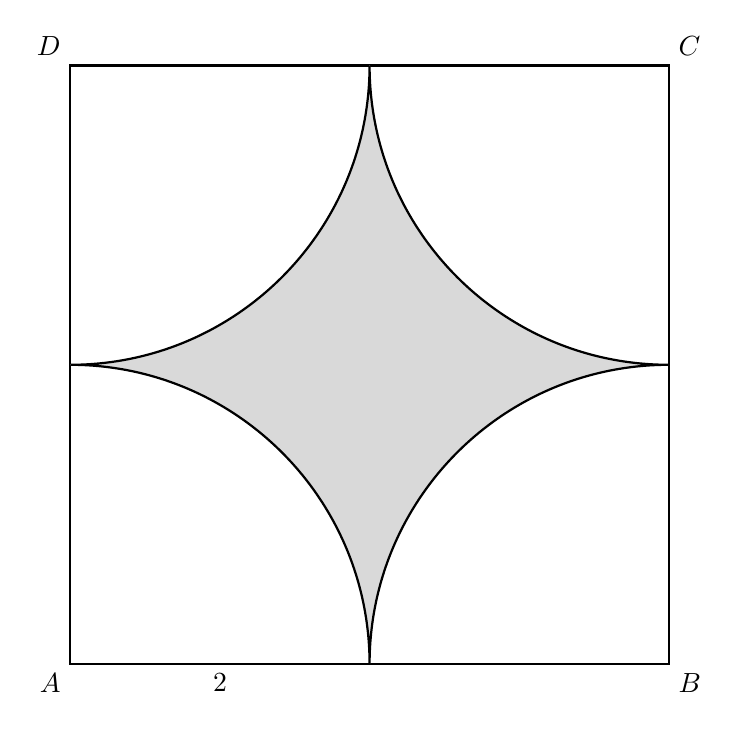
\begin{tikzpicture}[scale=1.9]
        \draw[thick] (0,0) rectangle (4,4);
        \node[below left] at (0,0) {$A$};
        \node[below right] at (4,0) {$B$};
        \node[above right] at (4,4) {$C$};
        \node[above left] at (0,4) {$D$};

        \filldraw[gray!30] (2,0) arc(0:90:2) arc(270:360:2) arc(180:270:2) arc(90:180:2);
        \draw[thick] (2,0) arc(0:90:2) arc(270:360:2) arc(180:270:2) arc(90:180:2);

        \draw[dashed] (0,0) -- (2,0);
        \node[below] at (1,0) {$2$};
    \end{tikzpicture}

\end{center}

    \begin{enumerate}[label=(\alph*)]
        \item 阴影部分的周长。（答案以$\pi$表示) \hfill (5\%)
        \item 阴影部分面积。（答案以$\pi$表示) \hfill (5\%)
    \end{enumerate}
\end{question}

\begin{solution}
    \begin{enumerate}[label=(\alph*)]
        \item 求阴影部分的周长（答案以 $\pi$ 表示）。 \\
        半径 $r=\dfrac{4}{2}=2\text{ cm}$，每段圆弧为 $\dfrac{1}{4}$ 圆周，共四段。
        \[
            \text{单段弧长} = \frac{90}{360}\times2\pi r = \pi \text{ (cm)}
        \]
        \hfill (2分)
        \[
            \text{总弧长} = 4\pi \text{ (cm)}
        \]
        \hfill (3分)

        \item 求阴影部分面积（答案以 $\pi$ 表示）。 \\
        阴影面积 $=$ 正方形面积 $-$ 四个 $\frac{1}{4}$ 圆的面积（四个 $\frac{1}{4}$ 圆彼此仅相切、互不重叠）。
        \[
            \frac{1}{4}\pi r^2 \times 4 = \pi \times 4 = 4\pi \text{ (cm}^2\text{)}
        \]
        \hfill (2分)
        \[
            16 - 4\pi \text{ (cm}^2\text{)}
        \]
        \hfill (3分)
    \end{enumerate}
\end{solution}
%endregion

%region 范围：初中数学-四边形与三角形的面积 | 考点：菱形面积、梯形面积逆运算、平行四边形与内接三角形面积之比 | 难度：中等
\begin{question}[points = 12]
    \begin{enumerate}[label=(\alph*)]
        \item 如下图所示，菱形 $ABCD$ 的两条对角线 $AC=10\text{ cm}$，$BD=7\text{ cm}$。求菱形 $ABCD$ 的面积。

        \begin{center}
        \begin{tikzpicture}[scale=0.6]
            \coordinate (A) at (0,5);
            \coordinate (C) at (0,-5);
            \coordinate (B) at (-3.5,0);
            \coordinate (D) at (3.5,0);
            \coordinate (O) at (0,0);
            \draw[thick] (A) -- (B) -- (C) -- (D) -- cycle;
            \draw[dashed] (A) -- (C);
            \draw[dashed] (B) -- (D);
            \pic[draw, angle radius=3mm] {right angle = A--O--D};
            \node[above] at (A) {$A$};
            \node[left] at (B) {$B$};
            \node[below] at (C) {$C$};
            \node[right] at (D) {$D$};
        \end{tikzpicture}
        \end{center} \hfill (4\%)

        \item 如下图所示，梯形 $EFGH$ 中 $EF \parallel HG$，$EF=8\text{ cm}$，梯形的高为 $6\text{ cm}$，梯形 $EFGH$ 的面积为 $66\text{ cm}^2$。求 $HG$ 的长。

        \begin{center}
        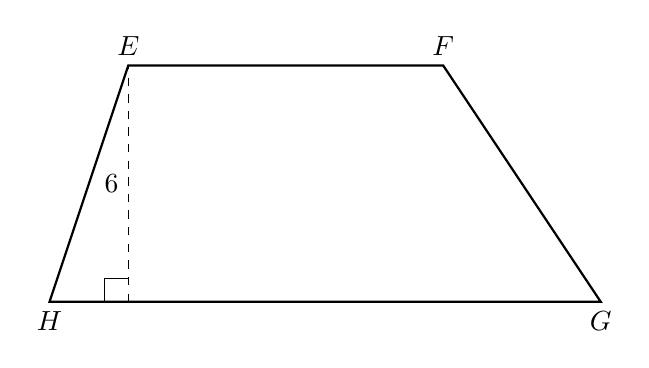
\begin{tikzpicture}[scale=0.5]
            \coordinate (E) at (2,6);
            \coordinate (F) at (10,6);
            \coordinate (G) at (14,0);
            \coordinate (H) at (0,0);
            \coordinate (K) at (2,0);
            \draw[thick] (E) -- (F) -- (G) -- (H) -- cycle;
            \draw[dashed] (K) -- (E);
            \pic[draw, angle radius=3mm] {right angle = E--K--H};
            \node[above] at (E) {$E$};
            \node[above] at (F) {$F$};
            \node[below] at (G) {$G$};
            \node[below] at (H) {$H$};
            \node[left] at (2,3) {$6$};
        \end{tikzpicture}
        \end{center} \hfill (5\%)

        \item 如下图所示，平行四边形 $JKLM$ 的底边 $JK=12\text{ cm}$，高为 $5\text{ cm}$。三角形 $JKN$ 内接于平行四边形 $JKLM$ 中，其中点 $N$ 在边 $LM$ 上。求 $\triangle JKN$ 的面积与平行四边形 $JKLM$ 的面积之比。

        \begin{center}
        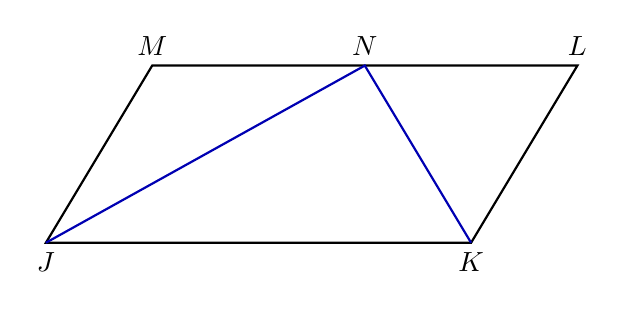
\begin{tikzpicture}[scale=0.45]
            \coordinate (J) at (0,0);
            \coordinate (K) at (12,0);
            \coordinate (L) at (15,5);
            \coordinate (M) at (3,5);
            \coordinate (N) at (9,5);
            \draw[thick] (J) -- (K) -- (L) -- (M) -- cycle;
            \draw[thick, blue!70!black] (J) -- (N) -- (K);
            \node[below] at (J) {$J$};
            \node[below] at (K) {$K$};
            \node[above] at (L) {$L$};
            \node[above] at (M) {$M$};
            \node[above] at (N) {$N$};
        \end{tikzpicture}
        \end{center} \hfill (4\%)
    \end{enumerate}
\end{question}

\begin{solution}
    \begin{enumerate}[label=(\alph*)]
        \item 已知菱形 $ABCD$ 对角线 $AC=10\text{ cm}$，$BD=7\text{ cm}$，求菱形面积。 \\
        菱形面积公式为对角线乘积的一半。
        \[
            S = \frac{1}{2}\times AC \times BD
        \]
        \hfill (2分)
        \[
            S = \frac{1}{2}\times10\times7 = 35 \text{ (cm}^2\text{)}
        \]
        \hfill (2分)

        \item 梯形 $EFGH$ 中 $EF\parallel HG$，$EF=8\text{ cm}$，高 $6\text{ cm}$，面积 $66\text{ cm}^2$，求 $HG$。 \\
        代入梯形面积公式，列方程求解。
        \[
            S = \frac{1}{2}\times(EF+HG)\times h
        \]
        \hfill (1分)
        \[
            66 = \frac{1}{2}\times(8+HG)\times6
        \]
        \hfill (1分)
        \[
            66 = 3\times(8+HG) \implies 22 = 8+HG
        \]
        \hfill (2分)
        \[
            HG = 14 \text{ (cm)}
        \]
        \hfill (1分)

        \item 平行四边形 $JKLM$ 底边 $JK=12\text{ cm}$，高 $5\text{ cm}$，$N$ 在 $LM$ 上，求 $\triangle JKN$ 与 $JKLM$ 的面积之比。 \\
        $\triangle JKN$ 与 $JKLM$ 同底 $JK$，且 $LM\parallel JK$，故同高，分别求面积后作比。
        \[
            S_{\triangle JKN} = \frac{1}{2}\times JK\times h = \frac{1}{2}\times12\times5 = 30 \text{ (cm}^2\text{)}
        \]
        \hfill (2分)
        \[
            S_{JKLM} = JK\times h = 12\times5 = 60 \text{ (cm}^2\text{)}
        \]
        \hfill (1分)
        \[
            S_{\triangle JKN} : S_{JKLM} = 30:60 = 1:2
        \]
        \hfill (1分)
    \end{enumerate}
\end{solution}
%endregion
\newpage


\vspace{1em}


\vfill % 与上方内容保持距离

\noindent
\newlength{\sigwidth}
\settowidth{\sigwidth}{（\hspace{4em}师）}

\begin{tabular*}{\textwidth}{@{\extracolsep{\fill}} l l l}
    出题： & 审题： & 审核： \\[4em]
    \rule{\sigwidth}{0.5pt} &
    \rule{\sigwidth}{0.5pt} &
    \rule{\sigwidth}{0.5pt} \\
    （\hspace{0em} \setterteacher ） &
    （\hspace{0em} \reviewteacher ） &
    （\hspace{0em} \auditteacher ） \\
\end{tabular*}

\newpage

\end{document}